
\chapter{Functional data structures}

This chapter describes more intricate details regarding more complex data structures, their representations in functional programs and their applications in the context of real-world problems.

\section{Combinator calculi}

Combinatory logic is a notation to eliminate the need for quantified variables in mathematical logic. It is based on \textit{combinators}, which were introduced by Schönfinkel with the idea of providing an analogous way to build up functions, and to remove any mention of variables. A combinator is a higher-order function that uses only function application and earlier defined combinators to define a result from its arguments. Implementation of various combinators in KamilaLisp is generally very straightfoward, due to the language's functional nature.

There are many different combinator calculi, but the SKI basis is used the most commonly. It is based on three combinators, \verb|S|, \verb|K| and \verb|I|, which are defined as follows:

\begin{itemize}
    \item \verb|S| is the \textit{substitution combinator}, which takes three arguments and applies the first to the second and third, then applies the result to the third argument. It is defined as \verb|(λ x y z . x z (y z))|.
    \item \verb|K| is the \textit{constant combinator}, which takes two arguments and returns the first one. It is defined as \verb|(λ x y . x)|.
    \item \verb|I| is the \textit{identity combinator}, which takes one argument and returns it. It is defined as \verb|(λ x . x)|.
\end{itemize}

These combinators can be used to define any other combinator, because the SKI basis is complete. It is important to note that the SK basis on its own would also be complete, since the I combinator can be written in the SK basis as follows:

\begin{Verbatim}
    SKK = (λ x y z . x z (y z)) (λ x y . x) (λ x y . x)
        = (λ x y x) (λ x x)
        = (λ x . x)
        = I
\end{Verbatim}

These definitions can be easily translated into KamilaLisp:

\begin{Verbatim}
    --> def S (λ x (λ y (λ z ((x z) (y z)))))
    (λ x . (λ y (λ z ((x z) (y z)))))
    --> def K (λ x (λ y x))
    (λ x . (λ y x))
    --> def I (λ x x)
    (λ x . x)
\end{Verbatim}

This allows for the further verification of the hypothesis that \verb|SKK = I|:

\begin{Verbatim}
    --> ((S K) K) 'a
    a
\end{Verbatim}

There are infinitely many combinators that can be expressed in the SK basis, a few of which are given below:

\begin{itemize}
    \item \verb|A| (apply) - \verb|SK(SK)| - \verb|λ a b . a b|, known as \verb|$| in Haskell.
    \item \verb|B| (bluebird) - \verb|S(KS)K| - \verb|λ a b c . a (b c)|, known as \verb|.| in Haskell.
    \item \verb|C| (cardinal) - \verb|S(BBS)(KK)| - \verb|λ a b c . a c b|, known as \verb|flip| in Haskell.
    \item \verb|T| (thrush) - \verb|CI| - \verb|λ a b . b a|, known as \verb|(&)| in Haskell.
    \item \verb|R| (robin) - \verb|BBT| - \verb|λ a b c . b c a|.
\end{itemize}

Three particularly interesting combinators are the $\omega$, $\Omega$ and Y combinators. The $\omega$ combinator is defined as \verb|λ x . x x|, primarily useful for duplicating a function, for example:

\begin{Verbatim}
    ω (λ x . x + 1) = (λ x . x x) (λ x . x + 1)
                    = (λ x . x + 1) (λ x . x + 1)
                    = (λ x . (x + 1) + 1)
                    = λ x . x + 2
\end{Verbatim}

The $\Omega$ combinator is defined as \verb|ω ω = (λ x . x x) (λ x . x x)|. Consider an attempt at evaluating this expression:

\begin{Verbatim}
    Ω = ω ω = (λ x . x x) (λ x . x x) = (λ x . x x) (λ x . x x) = ...
\end{Verbatim}

It is clearly impossible to ascribe a value to this expression, since the attempts at $\beta$-reduction will be unsuccessful, which makes the $\Omega$ combinator a curious and instructive introduction to the concept of the \textit{fixed point combinator}.

In combinatory logic for computer science, a fixed-point combinator is a higher-order function that returns some fixed point of its argument function, if one exists. Intuitively, $\text{fix} f = f (\text{fix} f)$. The implementation of the fixed-point combinator that is of particular interest is the Y combinator. It is defined as follows:

\begin{Verbatim}
    Y = λ f . (λ x . f (x x)) (λ x . f (x x))
\end{Verbatim}

The most interesting thing about the Y combinator is that it can be used to formally define recursive functions in a notation that does not support recursion. Of course, \verb|Y Y| can not be ascribed a value per \verb|Y f = f (Y f)| and hence \verb|Y Y = Y (Y Y)|. Consider the following definition of the Y combinator in KamilaLisp:

\begin{Verbatim}
    --> defun Y f ((λ x \x x) (λ x \f \λ y \(x x) y))
    (λ f . ((λ x (x x)) (λ x (f (λ y ((x x) y))))))
\end{Verbatim}

This definition can be used to define a canonical example of a recursive function, the Ackermann function - earliest-discovered examples of a total computable function that is not primitive recursive:

$$
\begin{array}{lcl}
    \operatorname {A} (0,n)&=&n+1\\
    \operatorname {A} (m+1,0)&=&\operatorname {A} (m,1)\\
    \operatorname {A} (m+1,n+1)&=&\operatorname {A} (m,\operatorname {A} (m+1,n))
\end{array}
$$

The definition of the Ackermann function using the Y combinator in KamilaLisp is given by:

\begin{Verbatim}
    --> def A \Y (lambda f (lambda a
    ...   (if (= (car a) 0) (+ (cadr a) 1)
    ...     (if (= (cadr a) 0) (f \tie (- (car a) 1) 1)
    ...       (f \tie (- (car a) 1) (f \tie (car a) (- (cadr a) 1)))))))
\end{Verbatim}

The invocation requires putting the arguments in a list and passing it to the function:

\begin{Verbatim}
    --> A '(3 3)
    61
\end{Verbatim}

A simpler example would be the factorial function:

\begin{Verbatim}
    --> def fact \Y (lambda f (lambda x
    ...   (if (= x 0) 1 (* x \f (- x 1)))))
    --> fact 10
    3628800
\end{Verbatim}

An evaluator for SKI calculus can be written by merging together a few independent parts. Starting with a function that performs a single evaluation step on a properly parenthesised SKI expression:

\begin{Verbatim}
  (defun SKI-step x
    (match x
      (((S K) 'x) 'I)
      (((S (K (S K))) K) '(S K))
      (((S (K (S (S K)))) K) 'K)

      ((((S 'x) 'y) 'z) (tie (tie x z) (tie y z)))
      (((K 'x) 'y) x)
      ((I 'x) x)
      (('x 'y) (tie (SKI-step x) (SKI-step y)))
      ('x x)))
\end{Verbatim}

The evaluation function minds various special cases including \verb|SKx=I| and \verb|S(K(SK))K=SK|, as they are impossible to derive using standard term-rewriting combinator calculi $\beta$-reduction (rudimentary $\eta$-expansion would be required\footnote{Barendregt's "The Lambda Calculus" provides an extension to the CL theory with a list of 5 $A_\beta$ axioms. Corollary 7.3.15 states that CL + $A_\beta$ is equivalent to $\lambda$, hence in principle one can use only these laws to prove the special cases, however implementing this is beyond the scope of this book.}). The next step is to define a function that properly parenthesises a SKI expression:

\begin{Verbatim}
  (defun SKI-lp x
    (match (reverse x)
      (('a) (SKI-lp a))
      (('a '...as) (tie (SKI-lp (reverse as)) (SKI-lp a)))
      ('a a)))
\end{Verbatim}

The final step is to combine these functions and converge the step function:

\begin{Verbatim}
  (defun SKI x (converge SKI-step (SKI-lp x)))
\end{Verbatim}

Validity of the code can be rudimentarily verified by evaluating an expression with known result:

\begin{Verbatim}
    --> SKI '(S I I K)
    (K K)
    --> ; SIIK=((SI)I)K=(IK)(IK)=KK
\end{Verbatim}

\section{Church encoding}

In mathematics, Church encoding is a method of representing data and operators in the lambda calculus.

\subsection{Natural numbers}

The Church numerals are the representations of natural numbers under Church encoding. They can be easily defined in terms of iterated function composition:

$$
\begin{array}{r|l}
    {\text{Number}}&{\text{Function definition}}\\
    \hline
    0&0\ f\ x=x\\
    1&1\ f\ x=f\ x\\
    2&2\ f\ x=f\ (f\ x)\\
    3&3\ f\ x=f\ (f\ (f\ x))\\
    \vdots&\vdots \\
    n&n\ f\ x=f^{n}\ x
\end{array}
$$

This concept can be trivially translated into KamilaLisp. For example, the Church numerals for 0 and 3 are given by:

\begin{Verbatim}
    --> defun c0 f #0
    (λ f . #0)
    --> defun c3 f (λ x (f (f (f x))))
    (λ f . (λ x (f (f (f x)))))
\end{Verbatim}

To verify the correctness of this definition and further experiments with Church numerals, the following function is defined to convert an arbitrary Church-encoded numeral into a natural number:

\begin{Verbatim}
    --> defun nat f ((f $(+ 1)) 0)
    (λ f . ((f $(+ 1)) 0))
    --> nat c3
    3
\end{Verbatim}

This function utilises the fact that Church encoding is in fact identical to iterated function composition, hence the natural successor function \verb|$(+ 1)| can be applied to it with a starting value of \verb|0|. To obtain the Church numeral for any natural number, define the following \textit{successor} function:

\begin{Verbatim}
    --> defun succ x (λ f (λ a (f ((x f) a))))
    (λ x . (λ f (λ a (f ((x f) a)))))
\end{Verbatim}

Using these, it is possible to verify that \verb|succ(succ(0)) = 2|:

\begin{Verbatim}
    --> nat (succ (succ c0))
    2
\end{Verbatim}

Using these properties, it is possible to define a function that yields the Church-encoded numeral for any given natural number:

\begin{Verbatim}
    --> defun church n (if n (succ (&0 (- n 1))) c0)
    (λ n . (if n (succ (&0/syn (- n 1))) c0))
    --> nat (church 5)
    5
\end{Verbatim}

Before giving more examples of operations on Church numerals, it is important to point out that using the helper functions \verb|church| and \verb|nat| or built-in natural number arithmetic functions would completely defeat the purpose of Church encoding in the first place, hence they will be used only to verify concrete results, and not to define new functions.

Addition of Church numerals can be easily defined in terms of their composition as $f^{m+n}\ x = f^m (f^n x) $, arguing for two definitions - one using the \verb|succ| function and the other using the identity verbatim:

\begin{Verbatim}
    --> defun add (x y) ((x succ) y)
    (λ x y . ((x succ) y))
    --> nat (add (church 3) (church 5))
    8
    --> defun add (m n) (λ f (λ x ((m f) ((n f) x))))
    (λ m n . (λ f (λ x ((m f) ((n f) x)))))
    --> nat (add (church 6) (church 5))
    11
\end{Verbatim}

Multiplication of Chruch numbers follows the same rule, $f^{m\times n}\ x = f^m (f^n x)$. It is important to notice what role the function composition aspect of Church numerals plays in this definition: the function \verb|f| is applied to the result of the composition of \verb|n| copies of \verb|f|, which is then applied to \verb|x|. Notice how currying is used to avoid the need for explicit application of \verb|x|:

\begin{Verbatim}
    --> defun mul (m n) (λ f (m (n f)))
    (λ m n . (λ f (m (n f))))
    --> nat \mul (church 5) (church 6)
    30
\end{Verbatim}

Exponentiation follows the same rule and can be very succinctly defined as follows due to currying:

\begin{Verbatim}
    --> defun cexp (m n) (n m)
    (λ m n . (n m))
    --> nat \cexp (church 5) (church 3)
    125
\end{Verbatim}

Subtraction is considerably more difficult to define. The natural numbers form a commutative monoid $(\mathbb{N}, +, 0)$. A binary relation $\sim$ on this monoid is defined as $m\sim n$ if and only if $m = n + k$ for some $k \in \mathbb{N}$. $\sim$ is obviously reflexive and transitive, while $\mathbb{N}$ is also naturally ordered since $\sim$ is also antisymmetric, making it a partial order. Furthermore, for all pairs of elements $a \in \mathbb{N}$ and $b \in \mathbb{N}$ there exists a unique smallest element $k$ such that $a \sim b + k$, hence $\mathbb{N}$ is a commutative monoid with monus, $a\ \dot -\ b$ of any two elements $a$ and $b$, which can be defined as this unique smallest element $k$ such that $a \sim b + k$. In $\mathbb{N}$ the monus operator is a saturating variant of standard subtraction between two integers such that $a\ \dot -\ b = \max(a - b, 0)$. 

To implement saturating subtraction, a predecessor function needs to be defined such that $\text{pred}(0) = 0$ and $\text{pred}(n + 1) = n$ for all $n \in \mathbb{N}$, hence the predecessor function must return a function that applies its parameter $n - 1$ times. This is achieved by building a container around $f$ and $x$, which is initialized in a way that omits the application of the function the first time:

\begin{Verbatim}
    --> defun pred n (λ f (λ x (((n (λ g (λ h (h (g f))))) (λ u x)) (λ u u))))
    (λ n . (λ f (λ x (((n (λ g (λ h (h (g f))))) (λ u x)) (λ u u)))))
    --> nat (pred (church 5))
    4
\end{Verbatim}

This definition of \verb|pred| can be simplified using the K and I combinators, however it is required to define a new combinator \verb|F = λ a b c . c (b a)|, which can be written written in terms of B and T as \verb|B(B T)T|:

\begin{Verbatim}
    --> def F (λ a (λ b (λ c (c \b a))))
    (λ a b c . (c (b a)))
    --> defun pred x (λ f (λ a (((x (F f)) (K a)) I)))
    (λ x . (λ f (λ a (((x (F f)) (K a)) I))))
    --> nat (pred (church 5))
    4
    --> nat (pred (church 0))
    0
\end{Verbatim}

It is sufficient to apply the \verb|pred| function to a Church numeral $m$, $n$ times to obtain the Church numeral $m - n$. Once again, this can be done by using currying and the fact that a Church numeral is essentially iterated application of a function:

\begin{Verbatim}
    --> defun sub (m n) ((n pred) m)
    (λ m n . ((n pred) m))
    --> nat (sub (church 5) (church 3))
    2
    --> nat (sub (church 3) (church 5))
    0
\end{Verbatim}

\subsection{Boolean domain}

Boolean numbers can also be encoded using Church encoding. It is perhaps not very surprising, since $\mathbb{B} = \{0, 1\}$, arguing for the following definitions of \verb|true| and \verb|false|:

\begin{Verbatim}
    --> defun bt f (λ x (f x))
    (λ f . (λ x (f x)))
    --> defun bf f (λ x x)
    (λ f . (λ x x))
\end{Verbatim}

However, it is more convenient to define them as combinators, so that \verb|T t f = t| and \verb|F t f = f|, which can be done as follows:

\begin{Verbatim}
    --> def T (λ t (λ f t))
    (λ t f . t)
    --> def F (λ t (λ f f))
    (λ t f . f)
\end{Verbatim}

This definition allows predicates (functions returning logical values) to directly act as \verb|if|-clauses. A function returning a Boolean, which is then applied to two parameters, returns either the first or the second parameter. Consequently, functions that convert between Church-encoded Booleans and standard natural numbers are given as follows:

\begin{Verbatim}
    --> defun b2n b ((b 1) 0)
    (λ b . ((b 1) 0))
    --> defun n2b n (if n T F)
    (λ n . (if n T F))
\end{Verbatim}

It is important to point out that \verb|true| and \verb|false| are defined canonically using the SK basis as \verb|T = K| and \verb|F = SK|. This definition allows for a particularly elegant definition of negation, as the \verb|t| and \verb|f| arguments are simply swapped:

\begin{Verbatim}
    --> defun bnot b ((b F) T)
    (λ b . ((b F) T))
    --> b2n \bnot T
    0
    --> b2n \bnot F
    1
\end{Verbatim}

To define negation in terms of the SKI basis it is sufficient to use the \verb|C| combinator, which is defined as \verb|C = λ a b c . a c b|, and written as \verb|S(BBS)(KK)|, which in turn $\beta$-reduces using the definition of \verb|B| to \verb|S(S(K(S(KS)K))S)(KK)|. The validity of this reasoning is verified when applying this expression to \verb|K| and \verb|SK|:

\begin{Verbatim}
    --> SKI '(S(S(K(S(K S)K))S)(K K) (S K))
    K
    --> SKI '(S(S(K(S(K S)K))S)(K K) K)
    (S K)
\end{Verbatim}

The next two operations to implement for Boolean values is logical AND and OR conjunctions:

\begin{Verbatim}
    --> defun bor x (λ y ((x T) y))
    (λ x . (λ y ((x T) y)))
    --> defun band x (λ y ((x y) F))
    (λ x . (λ y ((x y) F)))
\end{Verbatim}

Verify the truth tables:

\begin{Verbatim}
    --> defun tabulate f (discard \
    ...   :(lambda x \io:writeln \str:format
    ...     "{b2n \\car x} f {b2n \\cadr x} = {b2n \\(f (car x)) (cadr x)}")
    ...   (tie (tie T T) (tie T F) (tie F T) (tie F F)))
    --> tabulate bor
    1 f 1 = 1
    1 f 0 = 1
    0 f 1 = 1
    0 f 0 = 0
    --> tabulate band
    1 f 1 = 1
    1 f 0 = 0
    0 f 1 = 0
    0 f 0 = 0
\end{Verbatim}

Of course, the \verb|band| and \verb|bor| functions can also be written in the SKI basis. It is apparent that \verb|band = R(KI)| and \verb|bor = TK|. Per the definitions of these combinators:

\begin{Verbatim}
    band = R(KI)
         = (BBT)(KI)
         = (BB(CI))(KI)
         = (BB(S(BBS)(KK)I))(KI)
         = ((S(KS)K)(S(KS)K)(S((S(KS)K)(S(KS)K)S)(KK)I))(KI)
    bor  = TK
         = (CI)K
         = (S(BBS)(KK)I)K
         = (S((S(KS)K)(S(KS)K)S)(KK)I)K
\end{Verbatim}

\subsection{Natural number division and comparisons}

Elementary comparisons between Church-encoded natural numbers are rather straightforward. The following definitions of \verb|leq?| and \verb|zero?| are given as follows:

\begin{Verbatim}
    --> defun zero? n ((n (λ x F)) T)
    (λ n . ((n (λ x F)) T))
    --> defun leq? n (λ m (zero? (sub n m)))
    (λ n . (λ m (zero? (sub n m))))
\end{Verbatim}

The definition of \verb|zero?| uses the fact that a Church number greater than zero will iterate the function \verb|(λ x F)| at least once, while a zero (an identity function) will simply yield \verb|T|. The second function that utilises the monus operator uses \verb|sub| and \verb|zero?| to determine whether the first number is less than or equal to the second number. Defining equality involves computing the absolute difference between two numbers, given as $|a - b| = (x{ \dot -}y) + (y{ \dot -}x)$:

\begin{Verbatim}
    --> defun eq? n (λ m (zero? (add (sub n m) (sub m n))))
    (λ n . (λ m (zero? (add (sub n m) (sub m n)))))
\end{Verbatim}

Other kinds of inequalities can be defined using these functions as follows:

\begin{Verbatim}
    --> defun gt? n (λ m (bnot ((leq? n) m)))
    (λ n . (λ m (bnot ((leq? n) m))))
    --> defun lt? n (λ m ((gt? m) n))
    (λ n . (λ m ((gt? m) n)))
    --> defun geq? n (λ m (bnot ((lt? n) m)))
    (λ n . (λ m (bnot ((lt? n) m))))
\end{Verbatim}

Defining the division of Church-encoded natural numbers is considerably more involved than multiplication or exponentiation. To define division in $\mathbb{N}$, consider the numbers $a,b\in\mathbb{N}$ such that $b\ne 0$. It is apparent that in ${\displaystyle \exists_1 q, r \in \mathbb{N}: a = q b + r, r < b}$ where $q$ is the quotient and $r$ is the remainder. The following definition of division is based on this observation:

$$
n/m=\operatorname {if} \ n\geq m\ \operatorname {then} \ 1+(n-m)/m\ \operatorname {else} \ 0
$$

This mathematical definition can be easily written in KamilaLisp:

\begin{Verbatim}
    --> defun div n (λ m (((
    ...   ((geq? n) m)
    ...     (λ _ \succ ((div (sub n m)) m)))
    ...     (λ _ c0)) 'nil))
    --> nat \(div c6) c3
    2
    --> nat \(div c6) (succ (succ c0))
    3
    --> nat \(div c6) (succ c0)
    6
\end{Verbatim}

Curiously, division by zero overflows the stack:

\begin{Verbatim}
    --> (div c3) c0
    StackOverflowError thrown in thread 0X7ef82753:
        null
\end{Verbatim}

The definition of modulus can be easily conjectured using already implemented truncating division:

$$
n\text{ mod }m = n - (n/m) \cdot m
$$

Transcribing this definition into KamilaLisp:

\begin{Verbatim}
    --> defun cmod n (λ m (sub n (mul ((div n) m) m)))
    (λ n . (λ m (sub n (mul ((div n) m) m))))
    --> nat \(cmod c6) (succ c3)
    2
\end{Verbatim}

\subsection{Pairs}

Church pairs are the Church encoding of the pair type. The pair is represented as a function that takes a function argument. When given its argument it will apply the argument to the two components of the pair. The definition of Church pairs in KamilaLisp is as follows:

\begin{Verbatim}
    --> defun pair (x y) (λ f ((f x) y))
    (λ x y . (λ f ((f x) y)))
    --> def fst (λ p (p K))
    (λ p . (p K))
    --> def snd (λ p (p (K I)))
    (λ p . (p (K I)))
\end{Verbatim}

It is easy to verify the correctness of this approach:

\begin{Verbatim}
    --> fst (pair 'a 'b)
    a
    --> snd (pair 'a 'b)
    b
\end{Verbatim}

Pairs are canonically used in implementing signed Church numerals, where each signed Church numeral is a pair of two Church-encoded natural numbers, the first representing the positive part and the second representing the negative part. Consequently, rational numbers can be encoded as a pair of a signed Church numeral and a Church-encoded natural number, where the earlier represents the numerator, while latter represents the denominator. Using similar logic, it is also possible to encode computable real numbers, i.e. numbers that can be approximated by some computable function  $f\ :\ \mathbb{N} \to \mathbb{Z}$ such that given any $n \in \mathbb{N}$, the following holds:

$$ \frac{f(n) - 1}{n} \le a < \frac{f(n) + 1}{n} $$

Complex numbers are naturally encoded as a pair of real numbers.

\subsection{Lists}

Exploring the Church encoding for lists is particularly beneficial for encoding other, more complex data structures. In practice, a string can be encoded as a list of code points, a graph can be encoded as a list of edges, and a tree can be encoded as a list of nodes. This adheres to the Church-Turing thesis, a consequence of which is that any data type or calculation may be encoded in lambda calculus.

There are many ways to encode lists using the Church encoding. The most straightforward of them is to use pairs to build up a linked list. It is obvious that \verb|cons| can be defined as \verb|pair|, \verb|car| is \verb|fst|, \verb|cdr| is \verb|snd| and \verb|nil| is \verb|F|. \verb|cempty?| is thus defined as follows:

\begin{Verbatim}
    --> defun cempty? l ((l (λ h \λ t \λ d F)) T)
    (λ l . (l (λ _ F) T))
    --> b2n \cempty? F
    1
    --> b2n \cempty? (pair 'a (pair 'b F))
    0
\end{Verbatim}

Given these functions, it is possible to give recursive implementations of common list-related abstractions over recursion (\verb|map|, \verb|foldl|, \verb|foldr|, \verb|filter|, etc.).

The canonical way to represent a list in Church encoding is to define it as a right-fold with the \verb|cons| and \verb|nil| arguments, so that for example \verb|'(1 2 3)| becomes \verb|λ c n . c 1 (c 2 (c 3 n))|. \verb|nil| is particularly easy to define, as it merely returns the \verb|n| component of the argument pair:

\begin{Verbatim}
    --> def cnil (λ (c n) n)
    (λ c n . n)
\end{Verbatim}

\verb|ccons| is a function of an element \verb|x| and a list \verb|xs|, so that it yields \verb|λ c n . c x (xs c n)| - creating a new "cons cell" and setting its \verb|nil| value to the list:

\begin{Verbatim}
    --> defun ccons (x xs) (λ (c n) (c x (xs c n)))
    (λ x xs . (λ (c n) (c x (xs c n))))
\end{Verbatim}

Because this Church-encoded list is essentially a right-fold, it is easy to write functions that convert from Church-encoded lists to regular lists and vice versa:

\begin{Verbatim}
    --> defun to-list (l) (l cons 'nil)
    (λ l . (l cons 'nil))
    --> defun from-list (l) (foldr ccons cnil l)
    (λ l . (foldr ccons cnil l))
    --> to-list \ccons 'a \from-list '(b c)
    (a b c)
\end{Verbatim}

As demonstrated in Chapter 2, right-folds are extremely powerful and can be used to implement \verb|append|, \verb|map|, \verb|filter| and many other list processing devices. Implementations of \verb|append| and \verb|all| are presented below:

\begin{Verbatim}
    --> defun cappend (xs ys) (lambda (c n) (xs c (ys c n)))
    (λ xs ys . (lambda (c n) (xs c (ys c n))))
    --> to-list \cappend (from-list '(a b)) (from-list '(c d))
    (a b c d)
    --> defun call (xs p) (xs (lambda (x xs) (and (p x) xs)) true)
    (λ xs p . (xs (lambda (x xs) (and (p x) xs)) true))
    --> call (from-list '(1 2 3 4 5)) (lambda x (< x 5))
    0
    --> call (from-list '(1 2 3 4)) (lambda x (< x 5))
    1
\end{Verbatim}

\section{Sets}

Sets in KamilaLisp don't differ fundamentally from lists. KamilaLisp sets are \textit{ordered}, meaning that operations on them such as union, intersection, taking the unique values, etc... - are all performed in a deterministic manner. As a consequence, sets already inherit many useful list functions, such as \verb|map|, \verb|filter| and all sorts of folds. Functions specific to sets are demonstrated below:

\begin{Verbatim}
    --> union '(1 2 3 5 6) '(2 3 5 7)
    (1 2 3 5 6 7)
    --> intersection '(1 2 3 5 6) '(2 3 5 7)
    (2 3 5)
    --> unique '(1 2 3 5 6)
    (1 2 3 5 6)
    --> without '(1 2 3 5 6) '(5 6)
    (1 2 3)
    --> powerset '(1 2 3)
    [nil
     (1)
     (2)
     (1 2)
     (1 3)
     (2 3)
     (1 2 3)
     (3)]
\end{Verbatim}

Set insertion is admittedly not a built-in function, but it can be easily implemented using \verb|cons| and \verb|in?|:

\begin{Verbatim}
    --> defun set-insert (el set) (if (in? el set) set (cons el set))
    (λ el set . (if (in? el set) set (cons el set)))
    --> set-insert 5 '(1 2 3 4)
    (5 1 2 3 4)
    --> set-insert 5 '(1 2 3 4 5)
    (1 2 3 4 5)
\end{Verbatim}

\section{Queues}

Queues are implemented in KamilaLisp using lists. This section will focus primarily on LIFO\footnote{LIFO: Last-In-First-Out} queues, FIFO\footnote{FIFO: First-In-First-Out} queues and priority queues. KamilaLisp generally encourages ad-hoc implementations of queues, since the elementary operations on LIFO and FIFO queues can be trivially implemented using list processing functions. For example, \verb|pop-front| could be implemented as \verb|[tie car cdr]|, \verb|push-back| is just \verb|append| while \verb|push-front| is \verb|cons|. Because KamilaLisp internally equates lists and vectors, this approach generally exhibits good performance characteristics. It is however possible to implement FIFO queues using two stacks\footnote{As conventionally done in OCaml or Haskell, since a linked list can be inexpensively used as a FIFO stack.}: an \verb|inbox| and \verb|outbox|. This way pushing an element to the queue is merely adding an element to the \verb|inbox| FIFO stack, while popping from the queue reduces to popping from the outbox if it is non-empty. If the \verb|outbox| is empty, data from \verb|inbox| is transferred to \verb|outbox|:

\begin{Verbatim}
    --> defun alt-q-push (el q) (tie (cons el (car q)) (cadr q))
    --> defun alt-q-pop q (
    ...   if (empty? \cadr q)
    ...     (&0 \[tie cadr car] q)
    ...     ([tie car@cadr \tie car cdr@cadr] q))
\end{Verbatim}

The implementation of a priority queue is a bit more involved. While insertion into a priority queue could be implemented by simply appending the new element to the queue and sorting it according to the priorities, this would be a rather inefficient solution. Instead, the following implementation of priority queue insertion is suggested:

\begin{Verbatim}
    --> (defun insert-pq (q el)
    ...   \insert q el
    ...     \count (lambda x \< (car x) (car el)) q)
\end{Verbatim}

This function takes a priority queue \verb|q| and an element \verb|el| and inserts \verb|el| into \verb|q| at the correct position. The \verb|insert| function is a generic function that takes a list, an element and a position and inserts the element at the given position. The \verb|count| function in this scenario counts elements with priority smaller than the priority of \verb|el|.

One algorithm that particularly benefits from priority queues is \textit{Huffman coding}. Huffman coding is a lossless compression algorithm that uses a variable-length code to represent the most common symbols in a file. The algorithm is based on the observation that symbols that occur more frequently in a file can be represented with fewer bits than symbols that occur less frequently. The algorithm works by building a binary tree, where the leaves are the symbols in the file and the internal nodes are the sums of the frequencies of the symbols in the leaves below them. To implement Huffman coding, start by computing the frequencies of each symbol in a buffer \verb|buf| and sorting the symbols by the frequencies in descending order:

\begin{Verbatim}
    --> def freq-tab \:[tie tally@cadr car] \group buf
    --> def freq-sorted freq-tab$[grade-up \car%[1] freq-tab]
\end{Verbatim}

The next step is to define a function that performs a single iteration of the tree building algorithm. The two least common symbols are combined into a single symbol, which is then inserted into the list of symbols in the correct position with combined frequencies:

\begin{Verbatim}
    --> (defun huffman-step pq
    ...   \if (= 1 \tally pq) pq
    ...     \insert-pq (cddr pq)
    ...       \tie (+ (caar pq) (car@cadr pq))
    ...         (tie (cadr@car pq) (cadr@cadr pq)))
\end{Verbatim}

The Huffman tree can be finally built by converging the step function:

\begin{Verbatim}
    --> def huffman-tree \car@cdar \converge huffman-step freq-sorted
\end{Verbatim}

To encode symbols in the buffer using the huffman tree, it needs first be labelled with the bit sequences that represent the symbols. This is accomplished in the following way:

\begin{Verbatim}
    --> (defun tag (t code) (
    ...   if (= 0 \tally t)
    ...     (tie t (reverse code))
    ...     (append (tag (car t) (cons 0 code))
    ...             (tag (cadr t) (cons 1 code)))))
    --> (def huffman-tab \bipartition rank \tag huffman-tree 'nil)
\end{Verbatim}

Given the Huffman table, it is now possible to encode the buffer. Because Huffman codes are variable-length, it is important that the encoded buffer is padded with zeros to the nearest multiple of 8 to form a full byte. This is accomplished by the following function:

\begin{Verbatim}
    --> (def encoding-ids
          \flatten (car huffman-tab)$[$(car@index-of)%[0 1] (tie buf) (cdr huffman-tab)])
    --> def padded \take (bit:and (+ (tally encoding-ids) 7) -8) encoding-ids
\end{Verbatim}

Finally, instead of encoding all the auxiliary data into a buffer or file, for simplicity return the huffman table, encoded bits and the bit length verbatim:

\begin{Verbatim}
    --> (tie (tally encoding-ids) huffman-tab
          \:$(- _ 128)@:$(decode 2)
            \partition (cycle (tally padded) (take 8 '(1))) padded)
\end{Verbatim}

To reverse the encoding process, assume that \verb|buf| is now defined as the result above. First, the bit stream, bit length and huffman table are extracted from the buffer:

\begin{Verbatim}
    --> def bit-len (car buf)
    --> def huffman-table (cadr buf)
    --> (def bit-stream (take bit-len
    ...   \flatten@:(lambda x \reverse@take 8 \reverse@encode 2 (+ 128 x))
    ...     \car@cddr buf))
\end{Verbatim}

The step function that performs a single iteration of the decoding algorithm is defined as follows:

\begin{Verbatim}
    --> (defun unhuffman-step (stream dec) (let-seq
    ...   (def match-idx \car@where@:starts-with (tie stream) (car huffman-table))
    ...   (def match-len \tally (car huffman-table)$[#0 match-idx])
    ...   (def new-dec (append dec \tie (cadr huffman-table)$[#0 match-idx]))
    ...   (def new-stream (drop match-len stream))
    ...   (if (= 0 \tally new-stream) new-dec \&0 new-stream new-dec)))
\end{Verbatim}

First, the function finds the Huffman table entry index which is the prefix of the bit stream (\verb|match-idx|). Then the length of the prefix is computed. The decoded symbol is then appended to the decoded buffer and the prefix is dropped from the bit stream. The function is then recursively applied to the remaining bit stream and the new decoded buffer. Finally, the function is applied as follows:

\begin{Verbatim}
    --> unhuffman-step bit-stream 'nil
\end{Verbatim}

\section{Dictionaries}

KamilaLisp implements dictionaries as persistent maps. Like every other data structure in KamilaLisp, they are immutable. Dictionaries in KamilaLisp are chiefly used as key-value storage and in process of implementing prototype-based object orientation. The following example illustrates dictionary constructors:
\begin{Verbatim}
    --> def fruits %{
    ...   "apple" => "Apfel",
    ...   "pear" => "Birne",
    ...   "apricot" => "Aprikose"
    ... }
    --> def digits %{
    ...   1 => '("Ein" "One"),
    ...   2 => '("Zwei" "Two"),
    ...   3 => '("Drei" "Three"),
    ...   4 => '("Vier" "Four")
    ... }
\end{Verbatim}

It is important to emphasise that KamilaLisp primarily employs \textit{data constructors}, not \textit{literals}. This means that the dictionary constructors demonstrated above are not literals, but rather functions with special syntax that return dictionaries. The only way to create a \textit{literal} is to quote data. The difference between data constructors and literals is illustrated on the following example:

\begin{Verbatim}
    --> def a 5
    5
    --> def my-map %{
    ...   a => 'a,
    ...   'a => 'a,
    ...   (+ a 5) => 'a
    ... }
    {5=a, 10=a, a=a}
\end{Verbatim}

Adding and removing data to and from dictionaries is done using the \verb|hashmap:adjoin| and \verb|hashmap:minus|. The following example illustrates the usage of these functions:

\begin{Verbatim}
    --> def fruits-b \hashmap:adjoin fruits "banana" "Banane"
    {"pear"="Birne", "apple"="Apfel", "banana"="Banane", "apricot"="Aprikose"}
    --> def digits-3 \hashmap:minus digits 3
    {1=("Ein" "One"), 2=("Zwei" "Two"), 4=("Vier" "Four")}
\end{Verbatim}

A dictionary can be turned into or created from a plain list using \verb|hashmap:as-list| and \verb|hashmap:from-list|, respectively:

\begin{Verbatim}
    --> hashmap:as-list digits
    ((1 ("Ein" "One")) (2 ("Zwei" "Two")) (3 ("Drei" "Three")) (4 ("Vier" "Four")))
    --> hashmap:from-list '(("one" "Ein") ("two" "Zwei"))
    {"one"="Ein", "two"="Zwei"}
\end{Verbatim}

The functions \verb|hashmap:contains-key?| and \verb|hashmap:contains-value?| can be used to check whether a dictionary contains a given key or value:

\begin{Verbatim}
    --> hashmap:contains-key? digits 3
    1
    --> hashmap:contains-value? digits '("Drei" "Three")
    1
    --> hashmap:contains-key? digits-3 3
    0
    --> hashmap:contains-value? digits-3 '("Drei" "Three")
    0
\end{Verbatim}

There are three different ways to query values from a dictionary. The first, general way allows to query a dictionary for a given key using \verb|hashmap:get| and return \verb|nil| if the key is not present in the dictionary. The second way is to use \verb|hashmap:get-or| which returns the given default value if the key is not present in the dictionary. The last way is to use the dot operator to query the value of a given key of type \verb|string|. The following example illustrates the usage of all these approaches:

\begin{Verbatim}
    --> hashmap:get digits 3
    ["Drei"
     "Three"]
    --> hashmap:get digits 5
    --> hashmap:get-or digits 5 '("Funf" "Five")
    ["Funf"
     "Five"]
    --> ?my-dict.pear
    Birne
    --> ?my-dict.apple
    Apfel
    --> ?my-dict.potato
\end{Verbatim}

Dictionaries also implement a modified version of \verb|group| that groups the values of a list and creates a dictionary from the result. The following example illustrates the usage of this functionality:

\begin{Verbatim}
    --> def data '("apple" "pear" "apple" "pear" "pear" "apricot")
    ["apple"
     "pear"
     "apple"
     "pear"
     "pear"
     "apricot"]
    --> hashmap:group data
    {"pear"=(1 3 4), "apple"=(0 2), "apricot"=(5)}
\end{Verbatim}

Merging and subtracting dictionaries is performed using the \verb|hashmap:merge| and \verb|hashmap:without| functions. When merging, existing keys are overwritten. When subtracting, keys from the second dictionary that are present in the first dictionary are removed.

\begin{Verbatim}
    --> hashmap:merge %{1 => 2, 3 => 4} %{1 => 3, 2 => 6}
    {1=3, 2=6, 3=4}
    --> hashmap:without %{1 => 2, 3 => 4} %{1 => 3, 2 => 6}
    {3=4}
\end{Verbatim}

Finally, maps can be turned into a list of keys or a list of values using \verb|hashmap:key-list| and \verb|hashmap:value-list|, respectively:

\begin{Verbatim}
    --> hashmap:key-list fruits
    ["pear"
     "apple"
     "apricot"]
    --> hashmap:value-list fruits
    ["Birne"
     "Apfel"
     "Aprikose"]
\end{Verbatim}

The joint key-value pairs from a dictionary can be processed using \verb|hashmap:process|:

\begin{Verbatim}
    --> hashmap:process %{1 => 1, 2 => 4, 3 => 9, 4 => 16} :[tie car $(* 2)@cadr]
    {1=2, 2=8, 3=18, 4=32}
\end{Verbatim}

\section{Relations}

Formally speaking, a (binary) relation $\sim$ over a set $X$ can be seen as a set of ordered pairs $(x, y)$ of members of $X$. The relation $\sim$ holds between $x$ and $y$ if $(x, y)$ is a member of $\sim$. In KamilaLisp, such relation can also be seen as a function $\sim : X \times X \rightarrow \mathbb{B}$, where $\sim(x, y) = 1$ if $(x, y)$ is a member of $\sim$ and $\sim(x, y) = 0$ otherwise. Generally speaking, it is impossible to ascribe properties to relations defined as a function on an infinite set (e.g. $\mathbb{R}$, like the built-in relations \verb|/=| or \verb|<|) without symbolic manipulation. When studying the properties of relations (reflexivity, transitivity, etc...) it is therefore vital to define a relation as a finite set of ordered pairs. It is also allowed for a binary relation to associate the elements of one set (the \textit{domain}) with the elements of another set (the \textit{codomain}). If this is the case, a binary relation over sets $X$ and $Y$ is an element of the power set $X\times Y$. Since the latter set is ordered by inclusion, each relation has a place in the lattice of subsets of $X\times Y$. A binary relation is called a homogeneous relation when $X = Y$. A binary relation is also called a heterogeneous relation when it is not necessary that $X = Y$. Union of relations is defined like the union of sets: if $\sim$ and $\sim'$ are relations over $X$, then $\sim \cup \sim' = \{(x,y):x\sim y \vee x \sim' y\}$. For example, the union of the relations \verb|<| and \verb|>| is the relation \verb|/=|. Intersection of relations follows the same pattern. If $\sim$ is a relation over $X$ and $Y$ and $\sim'$ is a relation over $Y$ and $Z$, then the composition of these relations - denoted $\sim \circ \sim'$ - is the relation over $X$ and $Z$ defined by $\displaystyle \sim \circ \sim' = \{(x,z):\exists_{y \in Y} x \sim y \wedge y \sim' z\}$. Consider two relations:

\begin{Verbatim}
    --> def ~1 '((1 2) (2 3) (3 4) (4 5) (5 6))
    --> def ~2 '((2 4) (3 6) (4 8) (5 10) (6 12))
\end{Verbatim}

The following function can be used to compute the composition of two relations:

\begin{Verbatim}
    --> defun r-compose (r1 r2) (
    ...   let* (r2x \:car r2)
    ...     \flatten \:(lambda x
    ...       \let* ((a b) x)
    ...         \:$(cons a)@:cadr r2$[find-idx r2x b]) r1)
    --> r-compose ~1 ~2
    [(1 4)
     (2 6)
     (3 8)
     (4 10)
     (5 12)]
\end{Verbatim}

Both of the relations do not need to be injective:

\begin{Verbatim}
    --> def ~1 '((1 1) (2 4) (3 9))
    --> def ~2 '((1 1) (1 -1) (4 2) (4 -2) (9 3) (9 -3))
    --> r-compose ~1 ~2
    [(1 1)
     (1 -1)
     (2 2)
     (2 -2)
     (3 3)
     (3 -3)]
\end{Verbatim}

An identity relation (the identity element for relation composition) for $n \in \mathbb{N}$ up to $m$ is given as \verb|:[⌿⊙⍧ #0 #0]∘⍳ m|.

If $\sim$ is a binary relation over sets $X$ and $Y$, then the converse of $\sim$ is the relation $\sim^T$ over $Y$ and $X$ defined by $\displaystyle \sim^T = \{(y,x):x\sim y\}$. Iff\footnote{If and only if.} a relation is symmetric it is also its own converse - for example, \verb|=| and \verb|/=| are their own converses. The relations \verb|<| and \verb|>| are mutually converses of each other. The converse of a relation can be trivially computed using \verb|:reverse|. In the monoid of binary endorelations on a set (with the binary operation on relations being the composition of relations), the converse relation does not satisfy the definition of an inverse from group theory. The converse relation does satisfy the (weaker) axioms of a semigroup with involution: $\left(L^T\right)^T=L$ and $(L\circ R)^T=R^T\circ L^T$ (distributive law). $R$ is a symmetric binary relation over $X$ and $Y$ iff $R^T = R$, thus $R = \{(a,b): a R b \Leftrightarrow b R a \}$, so $(a,b)\in R \Rightarrow (b,a)\in R$. This can be easily checked for using \verb|[same-elements #0 :reverse]|. Uniqueness properties (injectivity and functionality) are checked for using, respectively, \verb|[same-elements unique #0]@:car| and \verb|[same-elements unique #0]@:cadr|.

Homogenous relations have the following properties of particular interest:

\begin{itemize}
    \item Reflexivity: $x \sim x$ for all $x \in X$ - \verb|def reflexive? all@:(lift =)|.
    \item Irreflexivity: $x \sim x$ does not hold for any $x \in X$ - \verb|def irreflexive? none@:(lift =)|.
    \item Symmetric: $x \sim y$ implies $y \sim x$ - \verb|def symmetric? [same-elements #0 :reverse]|.
    \item Antisymmetric: $x \sim y$ and $y \sim x$ implies $x = y$ - in other words, unless $x = y$ then both $x \sim y$ and $y \sim x$ cannot hold - \verb|[not-same-elements #0 :reverse]@$(filter \lift /=)|.
    \item Asymmetric: if $x \sim y$ then $y \sim x$ does not hold - in other words, the relation must be antisymmetric and irreflexive.
    \item Transitive: if $x \sim y$ and $y \sim z$ then $x \sim z$ - \verb|def transitive? [all@:^in? tie@#0 \r-compose #0 #0]|.
\end{itemize}

The transitive closure of a binary relation $\sim$ on a set $X$ is the smallest relation on $X$ that contains $\sim$ and is transitive. "Smallest" is chiefly taken in its usual sense, of having the fewest related pairs. To begin solving this problem, start by turning the relation into a matrix using \verb|where-mask|. The next step is converging a function that finds a transitive closure using inner product with \verb|or| as the accumulation part and \verb|and| as the mapping part. The function \verb|transitive-closure| is defined as follows:

\begin{Verbatim}
    --> ; Pad a matrix with zeroes to make it square.
    --> ⍥← sqm m (○⊢¨
    ...   (○← xd (⍴ \⍎ m))
    ...   (○← yd (⍴ m))
    ...   (↕¨
    ...     ((< xd yd) \:(λ x \⍠ x \↑ (- yd xd) '(0)) m)
    ...     ((> xd yd) \⍠ m \⍉↩ (- xd yd) \⌿⊙⍧ \↑ xd '(0))
    ...     ((= xd yd) m)))
    --> ; Compute the transitive closure.
    --> ⍥← transitive-closure x (○⊢¨
    ...   (○← x \sqm \⍸¯¹ x)
    ...   (⍥← ∨○∧ m \$(⌿⊙← ∨)%[1] \⌼ ∧ m \⎕⍉ m)
    ...   (⍸ \→≡ [∨ ∨○∧ #0] x))
\end{Verbatim}

Implementing the reflexive closure - the smallest relation on $X$ that contains $\sim$ and is reflexive - is considerably simpler and accomplished by \verb|:[tie #0 #0]@unique@flatten|.

\section{Graphs}

A graph is a data structure consisting of a set of objects (vertices) in which some pairs of the objects are related (linked). It is important to recognise how graphs are more general than trees - a tree is merely a connected undirected acyclic graph. The following elementary properties of graphs are considered:

\begin{itemize}
    \item A graph is either \textbf{directed} or \textbf{undirected}. This property specifies whether the links between vertices are ordered or not.
    \item A graph may be declared to contain \textbf{self-loops}. This property specifies whether a vertex may be linked to itself.
    \item A graph may be declared to contain \textbf{multiple edges}. This property specifies whether a vertex may be linked to another vertex more than once.
    \item A graph may be \textbf{weighted}, in which case each link is assigned a weight (a real number represented as a machine word; i.e. not arbitrary precision).
\end{itemize}

Depending on the declared properties of the graph, certain graphs are assigned names:

\begin{itemize}
    \item An undirected, unweighted graph with no self-loops and no multiple edges is called a \textbf{simple graph}.
    \item An undirected, unweighted graph with no self-loops and multiple edges is called a \textbf{multigraph}.
    \item An undirected, unweighted graph with that allows for self-loops and multiple edges is called a \textbf{pseudograph}.
\end{itemize}

Directed and weighted variants of these graphs exist, but they do not have unique names. For instance, a directed and weighted graph that allows for multiple edges but no self-loops will be referred to as a \textbf{directed and weighted multigraph}.

\subsection{Graph constructors}

Constructing a graph is done using the following KamilaLisp functions, all of which have similar interfaces explained later on in the book:

\begin{itemize}
    \item \verb|graph:simple| - constructs a simple graph.
    \item \verb|graph:simple-weighted| - constructs a weighted simple graph.
    \item \verb|graph:simple-directed| - constructs a directed simple graph.
    \item \verb|graph:simple-directed-weighted| - constructs a directed and weighted simple graph.
    \item \verb|graph:multi| - constructs a multigraph.
    \item \verb|graph:multi-weighted| - constructs a weighted multigraph.
    \item \verb|graph:multi-directed| - constructs a directed multigraph.
    \item \verb|graph:multi-directed-weighted| - constructs a directed and weighted multigraph.
    \item \verb|graph:pseudo| - constructs a pseudograph.
    \item \verb|graph:pseudo-weighted| - constructs a weighted pseudograph.
    \item \verb|graph:pseudo-directed| - constructs a directed pseudograph.
    \item \verb|graph:pseudo-directed-weighted| - constructs a directed and weighted pseudograph.
\end{itemize}

\par \noindent Constructing a graph requires specifying the edges and vertices:

\begin{Verbatim}
    --> def my-graph \graph:simple 
    ...   '(kamila lena julia anna diana)
    ...   '((diana anna) (kamila julia) (julia lena) (lena anna))

    Graph(
        Vertices=[kamila, lena, julia, anna, diana],
        Edges=[(diana => anna), (kamila => julia), (julia => lena), (lena => anna)]
    )
\end{Verbatim}

\subsection{Elementary graph operations}

The following elementary operations are defined on all graphs, regardless of their type.

\vspace{0.25cm} \par \noindent \verb|.has-vertex?| - checks whether a vertex is present in the graph.

\begin{Verbatim}
    --> my-graph.has-vertex? 'kamila
    1
    --> my-graph.has-vertex? 'jacob
    0
\end{Verbatim}

\par \noindent \verb|.has-edge?| - checks whether an edge is present in the graph.

\begin{Verbatim}
    --> my-graph.has-edge? '(lena anna)
    1
    --> my-graph.has-edge? '(lena kamila)
    0
\end{Verbatim}

\par \noindent \verb|.edges-of| - returns all the edges associated with a vertex.

\begin{Verbatim}
    --> my-graph.edges-of 'anna
    [(diana anna)
     (lena anna)]
\end{Verbatim}

\par \noindent \verb|.incoming-edges-of| - returns the set of all edges incoming into the specified vertex. This operation is only useful for directed graphs. For undirected graphs, it is equivalent to \verb|.edges-of|.

\vspace{0.25cm} \par \noindent \verb|.outgoing-edges-of| - returns the set of all edges outgoing from the specified vertex. This operation is only useful for directed graphs. For undirected graphs, it is equivalent to \verb|.edges-of|.

\vspace{0.25cm} \par \noindent \verb|.adjoin-vertex| - adds a vertex to the graph.

\begin{Verbatim}
    --> def graph2 \my-graph.adjoin-vertex 'rose
    Graph(
        Vertices=[kamila, lena, julia, anna, diana, rose],
        Edges=[(diana => anna), (kamila => julia), (julia => lena), (lena => anna)]
    )
\end{Verbatim}

\par \noindent \verb|.adjoin-edge| - adds an edge to the graph.

\begin{Verbatim}
    --> def graph2 \graph2.adjoin-edge '(rose lena)
    Graph(
        Vertices=[kamila, lena, julia, anna, diana, rose],
        Edges=[(diana => anna), (kamila => julia), (julia => lena),
               (lena => anna), (rose => lena)]
    )
\end{Verbatim}

\par \noindent \verb|.degree-of| - returns the degree of a vertex. The degree of a vertex is the number of edges incident to it.

\begin{Verbatim}
    --> graph2.degree-of 'lena
    3
\end{Verbatim}

\par \noindent \verb|.minus-edge| and \verb|.minus-vertex| operate in a similar fashion to \verb|.adjoin-edge| and \verb|.adjoin-vertex|, but they remove the specified edge or vertex from the graph. If the specified edge or vertex is not present in the graph, the graph is returned unchanged.

\vspace{0.25cm} \par \noindent \verb|.adjoin-edge-set|, \verb|.adjoin-vertex-set|, \verb|.minus-vertex-set|, \verb|.minus-edge-set| perform operations analogical to the ones described above, but work in batches by adjoining multiple edges or vertices, or removing multiple edges or vertices.

\subsection{Breadth-First and Depth-First Search}

Define a graph object that will be subsequently searched:

\begin{Verbatim}
    --> def my-graph \graph:simple-directed
        '(a b c d e f g h i j k)
        '((a b) (a c) (a d) (b e) (b f) (e g) (e h) (d i) (i j) (i k))
\end{Verbatim}

Which is represented as the following tree:

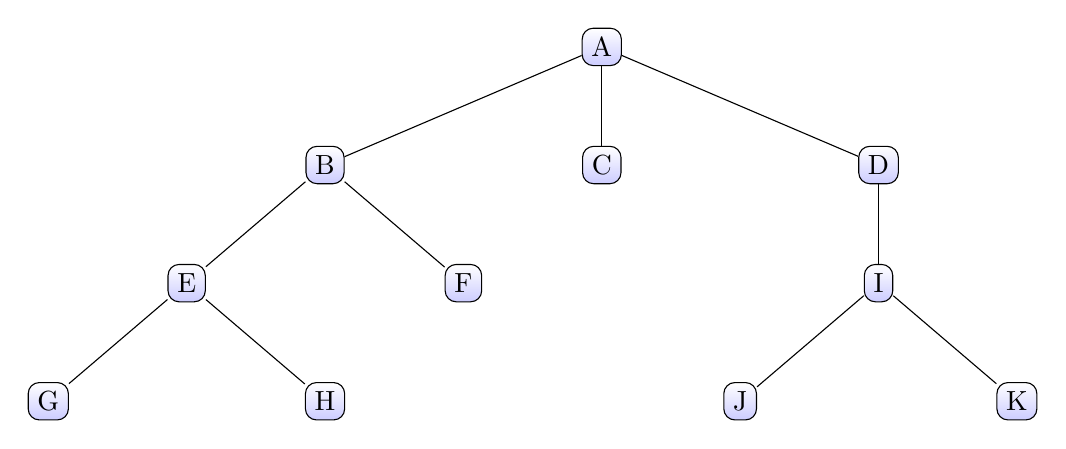
\begin{tikzpicture}[sibling distance=10em,
    every node/.style = {shape=rectangle, rounded corners,
      draw, align=center,
      top color=white, bottom color=blue!20}]
    \node {A}
      child { node {B} child { node{E} child { node{G} } child { node{H} } } child { node {F} } }
      child { node {C} }
      child { node {D} child { node {I} child { node {J} } child { node {K} } }};
\end{tikzpicture}





